% Options for packages loaded elsewhere
% Options for packages loaded elsewhere
\PassOptionsToPackage{unicode}{hyperref}
\PassOptionsToPackage{hyphens}{url}
\PassOptionsToPackage{dvipsnames,svgnames,x11names}{xcolor}
%
\documentclass[
  letterpaper,
  DIV=11,
  numbers=noendperiod]{scrartcl}
\usepackage{xcolor}
\usepackage{amsmath,amssymb}
\setcounter{secnumdepth}{-\maxdimen} % remove section numbering
\usepackage{iftex}
\ifPDFTeX
  \usepackage[T1]{fontenc}
  \usepackage[utf8]{inputenc}
  \usepackage{textcomp} % provide euro and other symbols
\else % if luatex or xetex
  \usepackage{unicode-math} % this also loads fontspec
  \defaultfontfeatures{Scale=MatchLowercase}
  \defaultfontfeatures[\rmfamily]{Ligatures=TeX,Scale=1}
\fi
\usepackage{lmodern}
\ifPDFTeX\else
  % xetex/luatex font selection
\fi
% Use upquote if available, for straight quotes in verbatim environments
\IfFileExists{upquote.sty}{\usepackage{upquote}}{}
\IfFileExists{microtype.sty}{% use microtype if available
  \usepackage[]{microtype}
  \UseMicrotypeSet[protrusion]{basicmath} % disable protrusion for tt fonts
}{}
\makeatletter
\@ifundefined{KOMAClassName}{% if non-KOMA class
  \IfFileExists{parskip.sty}{%
    \usepackage{parskip}
  }{% else
    \setlength{\parindent}{0pt}
    \setlength{\parskip}{6pt plus 2pt minus 1pt}}
}{% if KOMA class
  \KOMAoptions{parskip=half}}
\makeatother
% Make \paragraph and \subparagraph free-standing
\makeatletter
\ifx\paragraph\undefined\else
  \let\oldparagraph\paragraph
  \renewcommand{\paragraph}{
    \@ifstar
      \xxxParagraphStar
      \xxxParagraphNoStar
  }
  \newcommand{\xxxParagraphStar}[1]{\oldparagraph*{#1}\mbox{}}
  \newcommand{\xxxParagraphNoStar}[1]{\oldparagraph{#1}\mbox{}}
\fi
\ifx\subparagraph\undefined\else
  \let\oldsubparagraph\subparagraph
  \renewcommand{\subparagraph}{
    \@ifstar
      \xxxSubParagraphStar
      \xxxSubParagraphNoStar
  }
  \newcommand{\xxxSubParagraphStar}[1]{\oldsubparagraph*{#1}\mbox{}}
  \newcommand{\xxxSubParagraphNoStar}[1]{\oldsubparagraph{#1}\mbox{}}
\fi
\makeatother


\usepackage{longtable,booktabs,array}
\newcounter{none} % for unnumbered tables
\usepackage{calc} % for calculating minipage widths
% Correct order of tables after \paragraph or \subparagraph
\usepackage{etoolbox}
\makeatletter
\patchcmd\longtable{\par}{\if@noskipsec\mbox{}\fi\par}{}{}
\makeatother
% Allow footnotes in longtable head/foot
\IfFileExists{footnotehyper.sty}{\usepackage{footnotehyper}}{\usepackage{footnote}}
\makesavenoteenv{longtable}
\usepackage{graphicx}
\makeatletter
\newsavebox\pandoc@box
\newcommand*\pandocbounded[1]{% scales image to fit in text height/width
  \sbox\pandoc@box{#1}%
  \Gscale@div\@tempa{\textheight}{\dimexpr\ht\pandoc@box+\dp\pandoc@box\relax}%
  \Gscale@div\@tempb{\linewidth}{\wd\pandoc@box}%
  \ifdim\@tempb\p@<\@tempa\p@\let\@tempa\@tempb\fi% select the smaller of both
  \ifdim\@tempa\p@<\p@\scalebox{\@tempa}{\usebox\pandoc@box}%
  \else\usebox{\pandoc@box}%
  \fi%
}
% Set default figure placement to htbp
\def\fps@figure{htbp}
\makeatother





\setlength{\emergencystretch}{3em} % prevent overfull lines

\providecommand{\tightlist}{%
  \setlength{\itemsep}{0pt}\setlength{\parskip}{0pt}}



 


\KOMAoption{captions}{tableheading}
\usepackage{float}
\makeatletter
\@ifpackageloaded{caption}{}{\usepackage{caption}}
\AtBeginDocument{%
\ifdefined\contentsname
  \renewcommand*\contentsname{Table of contents}
\else
  \newcommand\contentsname{Table of contents}
\fi
\ifdefined\listfigurename
  \renewcommand*\listfigurename{List of Figures}
\else
  \newcommand\listfigurename{List of Figures}
\fi
\ifdefined\listtablename
  \renewcommand*\listtablename{List of Tables}
\else
  \newcommand\listtablename{List of Tables}
\fi
\ifdefined\figurename
  \renewcommand*\figurename{Figure}
\else
  \newcommand\figurename{Figure}
\fi
\ifdefined\tablename
  \renewcommand*\tablename{Table}
\else
  \newcommand\tablename{Table}
\fi
}
\@ifpackageloaded{float}{}{\usepackage{float}}
\floatstyle{ruled}
\@ifundefined{c@chapter}{\newfloat{codelisting}{h}{lop}}{\newfloat{codelisting}{h}{lop}[chapter]}
\floatname{codelisting}{Listing}
\newcommand*\listoflistings{\listof{codelisting}{List of Listings}}
\makeatother
\makeatletter
\makeatother
\makeatletter
\@ifpackageloaded{caption}{}{\usepackage{caption}}
\@ifpackageloaded{subcaption}{}{\usepackage{subcaption}}
\makeatother
\usepackage{bookmark}
\IfFileExists{xurl.sty}{\usepackage{xurl}}{} % add URL line breaks if available
\urlstyle{same}
\hypersetup{
  pdftitle={Etapa 2: Conociendo los datos},
  pdfauthor={Alicia Bernádez A01562634; Omar Arzaga A01569294; Diego Medrano A01254882; Sebastián Alemán A00841034; Isaac Montaño A00841681},
  colorlinks=true,
  linkcolor={blue},
  filecolor={Maroon},
  citecolor={Blue},
  urlcolor={Blue},
  pdfcreator={LaTeX via pandoc}}


\title{Etapa 2: Conociendo los datos}
\author{Alicia Bernádez A01562634 \and Omar Arzaga A01569294 \and Diego
Medrano A01254882 \and Sebastián Alemán A00841034 \and Isaac Montaño
A00841681}
\date{}
\begin{document}
\maketitle


\subsection{Objetivo del análisis}\label{objetivo-del-anuxe1lisis}

Analizar y caracterizar las concentraciones de dióxido de azufre
(\(SO_2\)) registradas durante 2022-2025 en las estaciones SE3
(Cadereyta), SE2 (Juárez), NE (San Nicolás) y GAR (García), así como su
relación con las condiciones meteorológicas, principalmente la dirección
y velocidad del viento, con el propósito de identificar patrones
espaciales y direccionales consistentes con una posible influencia de
fuentes industriales en la zona de Cadereyta.

\subsection{Técnicas estadísticas}\label{tuxe9cnicas-estaduxedsticas}

\paragraph{\texorpdfstring{1. Análisis espacio-temporal de
\(SO_2\)}{1. Análisis espacio-temporal de SO\_2}}\label{anuxe1lisis-espacio-temporal-de-so_2}

Esta técnica permitirá estudiar cómo cambian las concentraciones de
\(SO_2\) a través del tiempo y entre las distintas estaciones de
monitoreo. Se analizarán patrones por año, mes y hora, además de
comparar el comportamiento de las estaciones seleccionadas. Este tipo de
análisis ha sido utilizado en estudios de ciudades industriales para
identificar diferencias espaciales y temporales en los niveles de
contaminantes y reconocer episodios de concentraciones elevadas (Clarke
et al, 2014; Xue et al, 2023). En este proyecto permitirá determinar si
los valores altos de \(SO_2\) se concentran principalmente en
determinadas estaciones o periodos.

\paragraph{2. Gráficos polares
bivariados}\label{gruxe1ficos-polares-bivariados}

Los gráficos polares permiten analizar de manera conjunta la
concentración de un contaminante, la dirección del viento y su
velocidad. De esta forma, es posible identificar las condiciones del
viento bajo las cuales se presentan las mayores concentraciones de
\(SO_2\) y visualizar los sectores desde los que podrían transportarse
las emisiones hacia cada estación. Esta metodología ha sido aplicada
para diferenciar posibles contribuciones de distintas fuentes de
contaminación y se encuentra implementada en el paquete openair de R
(Carslaw et al, 2006; Carslaw \& Ropkins, 2012). En el presente estudio,
los patrones obtenidos podrán compararse con la ubicación geográfica de
la zona industrial de Cadereyta.

\paragraph{3. Conditional Bivariate Probability Function
(CBPF)}\label{conditional-bivariate-probability-function-cbpf}

La CBPF permite estimar la probabilidad d eobservar concentraciones
elevadas de un contaminante bajo diferentes combinaciones de dirección y
velocidad del viento. a diferencia del gráfico polar, que muestra
principalmente la magnitud de las concentraciones, esta técnica se
enfoca en identificar las condiciones meteorológicas asociadas con una
mayor frecuencia de valores elevados. La metodología extiende los
enfoques de probabilidad condicional utilizados previamente para la
identificación de regiones potencialmente emisoras (Ashbaugh et at,
1985; Uria-Tellaetxe \& Carslaw, 2014). Su aplicación permitirá
identificar sectores direccionales asociados con una mayor presencia de
concentraciones altas de \(SO_2\).

\paragraph{4. Caracterización comparativa de episodios
elevados}\label{caracterizaciuxf3n-comparativa-de-episodios-elevados}

Esta técnica podría contrbuir a identificar y comparar episodios de
concentraciones elevadas de \(SO_2\) considerando la estación donde
ocurren, las condiciones meteorológicas presentes y su posible
simultaneidad con otras estaciones. Su aplicación permitiría distinguir
entre eventos con un comportamiento más localizado y aquellos que se
presentan en varias zonas al mismo tiempo, lo cual podría ser indicativo
de fenómenos de mayor escala. Estudios previos han utilizado el análisis
individual de episodios de contamiación para explorar posibles fuentes y
condiciones asociadas con eventos recurrentes de \(SO_2\) (Clarke et al,
2014; Xue et al, 2023). De manera complementaria, durante estos
episodios también podría examinarse el comportamiento de otros
contaminantes, sin asumir que necesariamente deben presentar incrementos
simultáneos.

\subsection{Variables elegidas}\label{variables-elegidas}

Para responder al objetivo del proyecto se consideran como variables
principales la concentración de \(SO_2\), la dirección del viento (WDR),
la velocidad del viento (WSR) y la estación de monitoreo. También se
incluyen como variables meteorológicas complementarias la temperatura
exterior (TOUT), humedad relatica (RH), presión atmosférica (PRS),
radiación solar (SR) y precipitación (RAINF). Los demás contaminantes se
conservan como variables complementarias para caracterizar el contexto
de los registros de \(SO_2\).

\begin{table}[H]
\centering
\caption{Características descriptivas de SO$_2$ por estación}
\begin{tabular}{lrrrrr}
\hline
\textbf{Estación} & \textbf{Horas válidas} & \textbf{Media} & \textbf{Mediana} & \textbf{Desv. estándar} & \textbf{Máximo} \\
\hline
GAR & 32,534 & 3.48 & 3.30 & 1.25 & 22.80 \\
NE  & 33,185 & 4.35 & 3.80 & 2.96 & 163.60 \\
SE2 & 33,240 & 4.98 & 3.80 & 5.32 & 178.30 \\
SE3 & 33,977 & 7.25 & 4.40 & 11.00 & 404.70 \\
\hline
\end{tabular}
\end{table}

Descriptivamente, SE3 presenta las concentraciones medias y medianas de
\(SO_2\) más elevadas, así como la mayor variabilidad, mientras que GAR
presenta los valores más bajos y estables. Las cuatro estaciones cuentan
con cantidades similares de observaciones válidas, por lo que las
diferencias encontradas no parecen explicarse únicamente por una mayor
cantidad de datos en alguna estación. Estos resultados son exploratorios
y no permiten atribuir todavía las diferencias observadas a una fuente
específica.

\subsection{Gráficas}\label{gruxe1ficas}

\paragraph{\texorpdfstring{Boxplot de \(SO_2\) por
estación}{Boxplot de SO\_2 por estación}}\label{boxplot-de-so_2-por-estaciuxf3n}

\begin{figure}[H]

{\centering \pandocbounded{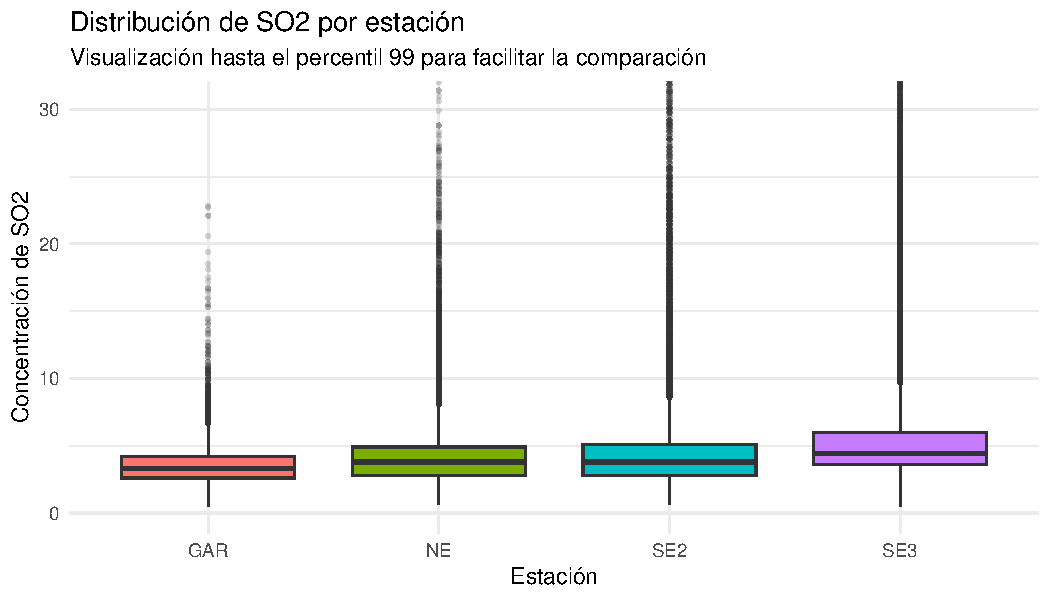
\includegraphics[keepaspectratio]{Etapa-2--Conociendo-los-datos_files/figure-pdf/unnamed-chunk-2-1.pdf}}

}

\caption{Distribución de SO2 por estación de monitoreo.}

\end{figure}%

\paragraph{\texorpdfstring{Histogramas de \(SO_2\) por
estación}{Histogramas de SO\_2 por estación}}\label{histogramas-de-so_2-por-estaciuxf3n}

\begin{figure}[H]

{\centering \pandocbounded{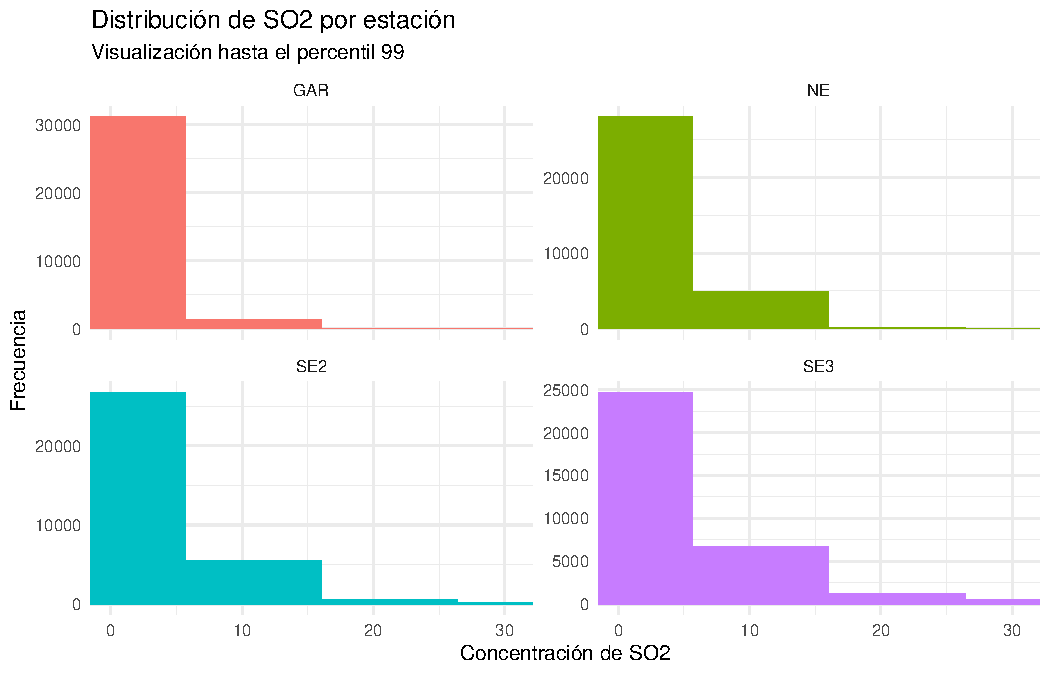
\includegraphics[keepaspectratio]{Etapa-2--Conociendo-los-datos_files/figure-pdf/unnamed-chunk-3-1.pdf}}

}

\caption{Distribución de las concentraciones de SO2 para cada estación.}

\end{figure}%

\paragraph{Matriz de correlación}\label{matriz-de-correlaciuxf3n}

\begin{figure}[H]

{\centering \pandocbounded{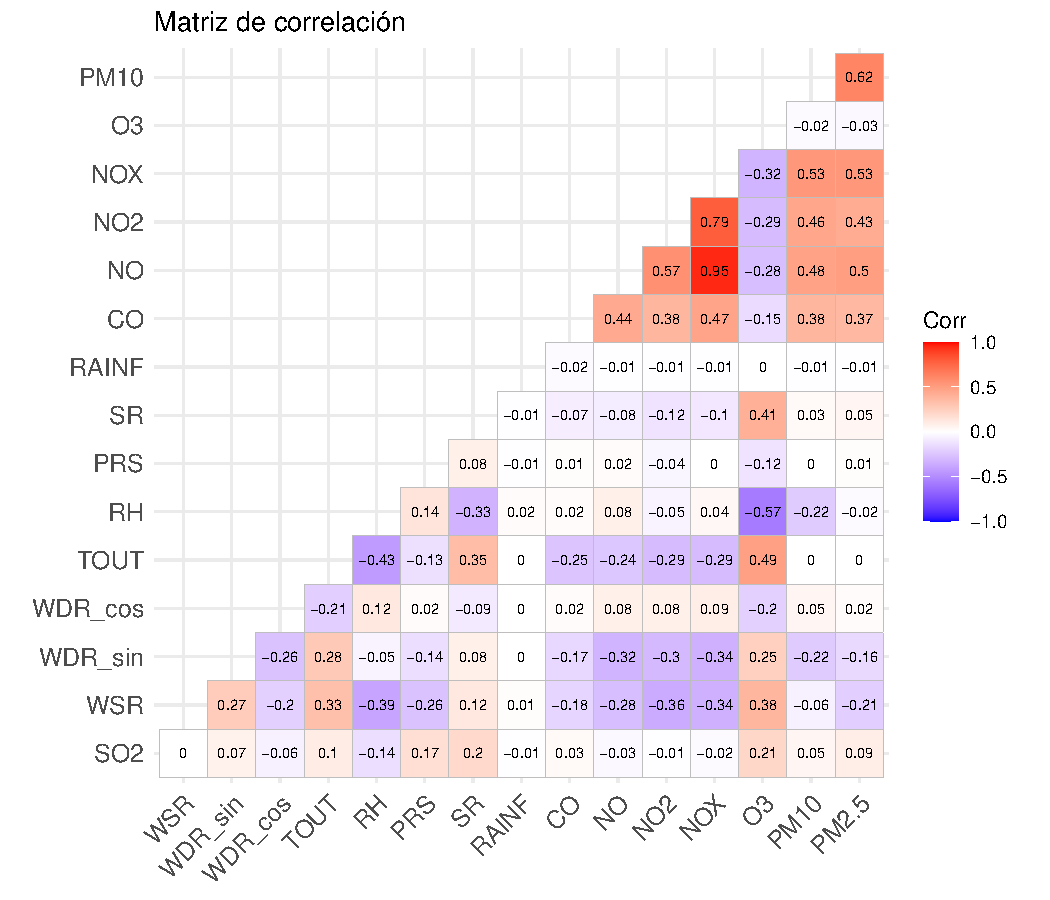
\includegraphics[keepaspectratio]{Etapa-2--Conociendo-los-datos_files/figure-pdf/unnamed-chunk-4-1.pdf}}

}

\caption{Matriz de correlación entre contaminantes y variables
meteorológicas.}

\end{figure}%

\paragraph{\texorpdfstring{Comportamiento anual de \(SO_2\) por
estación}{Comportamiento anual de SO\_2 por estación}}\label{comportamiento-anual-de-so_2-por-estaciuxf3n}

\begin{figure}[H]

{\centering \pandocbounded{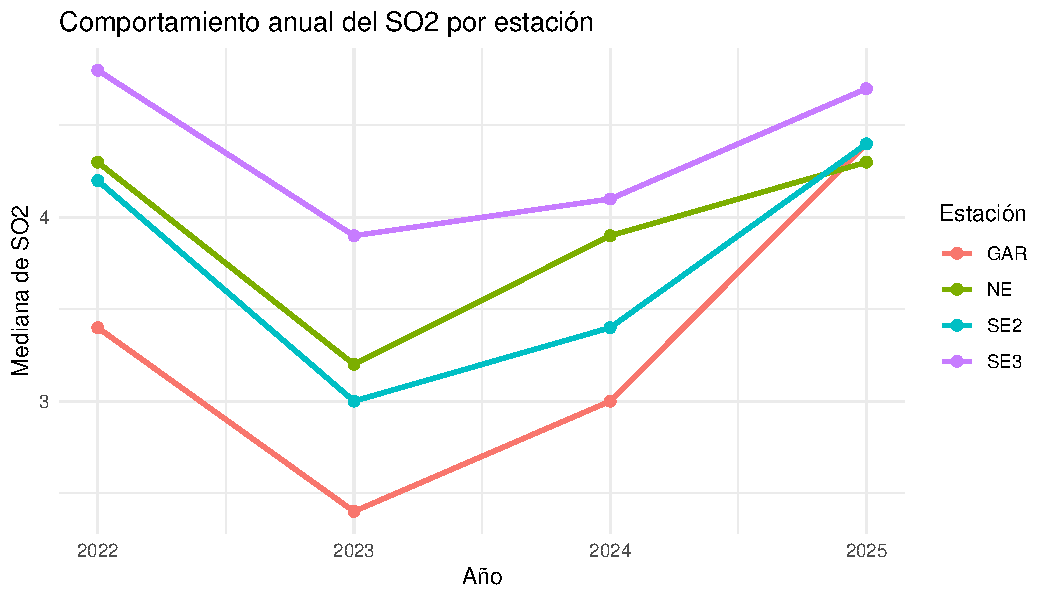
\includegraphics[keepaspectratio]{Etapa-2--Conociendo-los-datos_files/figure-pdf/unnamed-chunk-5-1.pdf}}

}

\caption{Comportamiento anual de la concentración mediana de SO2 por
estación.}

\end{figure}%

\subsection{Resumen}\label{resumen}

\subsection{Liga Github}\label{liga-github}

\subsection{Declaratoria de IA}\label{declaratoria-de-ia}

\begin{enumerate}
\def\labelenumi{\arabic{enumi}.}
\item
  Escribe, nuevamente, cuál es el objetivo de tu análisis. Si cambiaste
  de objetivo indica por qué. LISTO
\item
  Indica cuáles son las tecnicas estadísticas que contestarán tu
  objetivo (obtenlo de tu indagación bibliográfica previa) LISTO
\item
  Describe las variables que requieres para lograr tu objetivo y destaca
  sus principales características estadísticas. La estación de monitoreo
  es una variable importante.
\item
  Concluye con un breve resumen de lo que has logrado hasta ahora, qué
  falta por hacer, qué camino piensan seguir para lograrlo, cuáles son
  las preguntas que te han surgido, etc
\item
  No debe exceder de 5 páginas (incluyendo gráficas y tablas).
\item
  Incluye como anexos gráficos o tablas que creas conveniente mencionar
  en el texto que realizaste.
\item
  Inserta una liga (GitHub) que dé acceso a tu(s) documento(s) de
  trabajo y tu base de datos limpia (csv)
\item
  Incluye la declaratoria de uso de IA durante el desarrollo del
  trabajo:
\end{enumerate}




\end{document}
